\everymath{\displaystyle}
\documentclass{beamer}
% \documentclass[handout]{beamer}

%\usepackage[pdftex]{color,graphicx}
\usepackage{amsmath,amssymb,amsfonts}

\mode<presentation>
{
  % \usetheme{Darmstadt}
  % \usetheme[hideothersubsections]{Hannover}
  % \usetheme[hideothersubsections]{Goettingen}
  \usetheme[hideothersubsections, right]{Berkeley}

  \usecolortheme{seahorse}
  % \usecolortheme{dolphin}
  \usecolortheme{rose}
  % \usecolortheme{orchid}

  \useinnertheme[shadow]{rounded}

  \setbeamercovered{transparent}
  % or whatever (possibly just delete it)
}

\mode<handout>{
  \setbeamercolor{background canvas}{bg=black!5}
  \usepackage{pgfpages}
  \pgfpagesuselayout{4 on 1}[a4paper,border shrink=5mm, landscape]
}

\usepackage[brazilian]{babel}
% or whatever

% \usepackage[latin1]{inputenc}
\usepackage[utf8]{inputenc}
% or whatever

\usepackage{times}
%\usepackage[T1]{fontenc}
% Or whatever. Note that the encoding and the font should match. If T1
% does not look nice, try deleting the line with the fontenc.


\title%[] % (optional, use only with long paper titles)
{Tópicos de Escrita Científica}

\subtitle
{} % (optional)

\author%[] % (optional, use only with lots of authors)
{Felipe Figueiredo}% \and S.~Another\inst{2}}
% - Use the \inst{?} command only if the authors have different
%   affiliation.

\institute[INTO] % (optional, but mostly needed)
{Instituto Nacional de Traumatologia e Ortopedia
}
  % \inst{1}%
  % Department of Computer Science\\
  % University of Somewhere
  % \and
  % \inst{2}%
  % Department of Theoretical Philosophy\\
  % University of Elsewhere}
% - Use the \inst command only if there are several affiliations.
% - Keep it simple, no one is interested in your street address.

\date%[] % (optional)
{}

% \subject{Talks}
% This is only inserted into the PDF information catalog. Can be left
% out. 



% If you have a file called "university-logo-filename.xxx", where xxx
% is a graphic format that can be processed by latex or pdflatex,
% resp., then you can add a logo as follows:

\pgfdeclareimage[height=1.6cm]{university-logo}{../logo}
\logo{\pgfuseimage{university-logo}}



% Delete this, if you do not want the table of contents to pop up at
% the beginning of each subsection:
\AtBeginSubsection[]
%\AtBeginSection[]
{
  \begin{frame}<beamer>{Sumário}
    \tableofcontents[currentsection,currentsubsection]
  \end{frame}
}


% If you wish to uncover everything in a step-wise fashion, uncomment
% the following command: 

\beamerdefaultoverlayspecification{<+->}


\begin{document}

\begin{frame}
  \titlepage
\end{frame}

\begin{frame}{Sumário}
  \tableofcontents
  % You might wish to add the option [pausesections]
\end{frame}


%% Template
% \section{}

% \subsection{}

% \begin{frame}{}
%   \begin{itemize}
%   \item 
%   \end{itemize}
% \end{frame}

% \begin{frame}
%   \begin{columns}
%     \begin{column}{5cm}
%     \end{column}
%     \begin{column}{5cm}
%     \end{column}
%   \end{columns}
% \end{frame}

% \begin{frame}{}
%   \includegraphics[height=0.4\textheight]{file1}
%   \includegraphics[height=0.4\textheight]{file2}
%   \includegraphics[height=0.4\textheight]{file3}
%   \begin{figure}
%     \caption{}
%   \end{figure}
% \end{frame}

% \begin{frame}{}
%   \begin{definition}
%   \end{definition}
%   \begin{example}
%   \end{example}
%   \begin{block}{Exercício}
%   \end{block}
% \end{frame}

\section{Estrutura do texto}

\subsection{Expectativas do leitor}

\begin{frame}{As necessidades do leitor}
  \begin{block}{Gopen e Swan, 1990}
    ``Para o leitor apreender o que o autor quer dizer, o autor
    precisa entender o que o leitor precisa.''
  \end{block}
  \begin{block}{Hindle, 2013}
    ``Você não está escrevendo para você mesmo, está escrevendo para
    seu leitor.''
  \end{block}
  \begin{block}{Figueiredo, hoje.}
    ``O \alert{trabalho} da comunicação é seu, não do leitor.''
  \end{block}
\end{frame}

\begin{frame}
  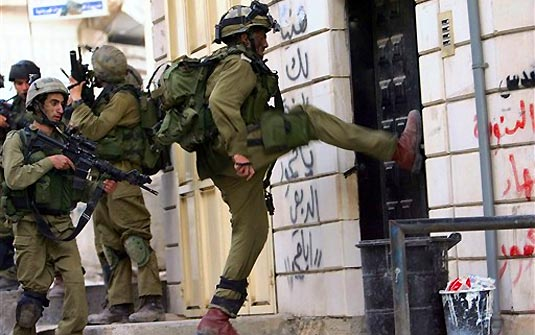
\includegraphics[width=\textwidth]{Escrita/penaporta}
\end{frame}
\begin{frame}{Exemplo}
  \begin{example}
    t(time)=15', T(temperature)=32$^o$C, t=0', T=25$^o$C; t=6',
    T=29$^o$C; t=3', T=27$^o$C; t=12', T=32$^o$C; t=9'; T=31$^o$C
  \end{example}

  \begin{itemize}
  \item Introduzir uma listagem de informações de forma textual pode
    ser oneroso para o leitor
  \item Especialmente se as medições não seguem uma ordem razoável
  \end{itemize}
\vfill
  Fonte: Gopen e Swan, 1990.
\end{frame}

\begin{frame}{Exemplo}
  \begin{example}
    \begin{tabular}{cc}
      time (min) & Temperature ($^o$C) \\
      0 & 25 \\
      3 & 27 \\
      6 & 29 \\
      9 & 31 \\
      12 & 32 \\
      15 & 32 \\
    \end{tabular}
  \end{example}
  \begin{itemize}
  \item<1-> Mesmas informações
  \item Mais facilidade para a compreensão do leitor
  \item \alert{Contexto} (tempo) onde cada \alert{informação}
    (temperatura) pode ser interpretada
  \end{itemize}
\vfill
  Fonte: Gopen e Swan, 1990.
\end{frame}

\begin{frame}{Exemplo}
  \begin{example}
    \begin{tabular}{cc}
      Temperature ($^o$C) & time (min) \\
      25 & 0 \\
      27 & 3 \\
      29 & 6\\
      31 & 9\\
      32 & 12\\
      32 & 15 \\
    \end{tabular}
  \end{example}
  \begin{itemize}
  \item A \alert{ordem} das informações faz diferença.
  \item Como lemos da esquerda para a direita, preferimos:
    \begin{enumerate}
    \item contexto na esquerda
    \item novidades na direita
    \end{enumerate}
  \end{itemize}

  \vfill
  Fonte: Gopen e Swan, 1990.
\end{frame}

\begin{frame}{Contexto $\times$ novidade}
  \begin{itemize}
  \item Todo texto científico começa com a Introdução, e termina com
    as Conclusões
  \item Isto também deve se aplicar às unidades textuais menores:
    \begin{enumerate}
    \item<2-> parágrafos
    \item<2-> frases
    \end{enumerate}
  \item O início da frase deve familiarizar o leitor
  \item O final da frase deve intrigar o leitor
  \end{itemize}
\end{frame}

\begin{frame}{Expectativas do leitor}
  \begin{itemize}
  \item Unidades textuais grandes (tese, dissertação, artigo, livro):
    \alert<-2>{expectativa} de localizar informação nas respectivas
    seções
  \item Seções confusas (eg. muitos detalhes experimentais em
    Resultados): leitor igualmente confuso
  \item Unidades menores (seção, parágrafo, frase): divisões menos
    óbvias, \alert<3>{expectativas estruturais persistem}
  \item Violação das expectativas: o \alert{leitor precisa dedicar
      energia} para decifrar a estrutura usada
  \item Resultado: risco de interpretação errônea, ou não compreensão
  \end{itemize}

\vfill
Gopen e Swan, 1990.
\end{frame}

\subsection{A posição de ênfase}

\begin{frame}{A posição de ênfase}
  \begin{example}
    \begin{itemize}
    \item Paul finalmente ganhou o prêmio depois de comprar 100
      bilhetes de loteria \alert<3->{na loja}.
    \item<4> Paul teve que comprar 100 bilhetes de loteria até finalmente
      \alert<5->{ganhar o prêmio}.
    \end{itemize}
  \end{example}

  \vfill
  Fonte: Wilke, 2013.
\end{frame}

\subsection{A posição de tópico}

\begin{frame}{A posição de tópico}
  \begin{example}
    A \alert<3->{erosão do solo} é um problema sério nas regiões
    montanhosas do Nepal.
  \end{example}
  \begin{block}{Assunto}
    O assunto da frase acima é a \alert<3->{erosão do solo}.
  \end{block}

  \vfill
  Fonte: Hindle, 2013.
\end{frame}

\begin{frame}{A posição de tópico}
  \begin{example}
    As \alert<3->{regiões montanhosas do Nepal} encaram problemas sérios com o
    aumento da erosão do solo.
  \end{example}
  \begin{block}{Assunto}
    Esta estrutura indica que o assunto da frase é \alert<3->{uma
      região específica} do Nepal.
  \end{block}

  \vfill
  Fonte: Hindle, 2013.
\end{frame}

\begin{frame}{Encadeamento de tópicos -- frase}
  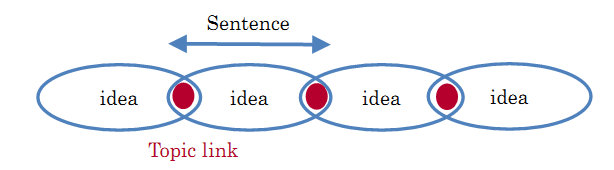
\includegraphics[width=\textwidth]{Escrita/encadeamento1}

  \vfill
  Fonte: Hindle, 2013.
\end{frame}

\begin{frame}{Encadeamento de tópicos -- parágrafos}
    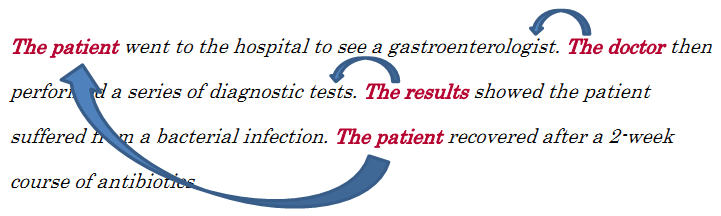
\includegraphics[width=\textwidth]{Escrita/encadeamento2}

  \vfill
  Fonte: Hindle, 2013.
\end{frame}

\subsection{Resumo}

\begin{frame}{Princípios estruturais}

  \begin{enumerate}
  \item Posicione o verbo após o sujeito gramatical tão cedo quanto
    possível
  \item Posicione a ``nova informação'' que você quer que o leitor
    enfatize na posição de ênfase
  \item Posicione a pessoa ou coisa a que a frase se refere no início,
    na posição de tópico.
  \item Posicione qualquer ``informação antiga'' (que já foi
    discutida) na posição de tópico para relacionar com o que passou e
    contextualizar com o que virá
  \item Articule a ação de cada frase em seu verbo.
  \item Em geral, indique algum contexto para seu leitor antes de
    exigir que ele considere qualquer informação nova
  \item Em geral, tente assegurar que as ênfases relativas do conteúdo
    coincidem com as expectativas relativas levantadas pela estrutura
  \end{enumerate}
\end{frame}

\begin{frame}{Referências}
  \begin{itemize}
  \item<1-> Gopen, George; Swan, Judith. The Science of Scientific
    Writing, 1990. American Scientist.
  \item<1-> Wilke, Claus. Writing paragraphs that make sense,
    2013. \url{http://serialmentor.com/blog/2013/9/26/writing-paragraphs-that-make-sensethe-topic-and-the-stress-position/}
  \item<1-> Hindle, Amanda. Reader expectations (blog series),
    2013. \url{http://www.edanzediting.com/blog/tag/reader_expectations}
  \end{itemize}
\end{frame}
\end{document}
